\chapter{Psalm 54}

\begin{figure}
  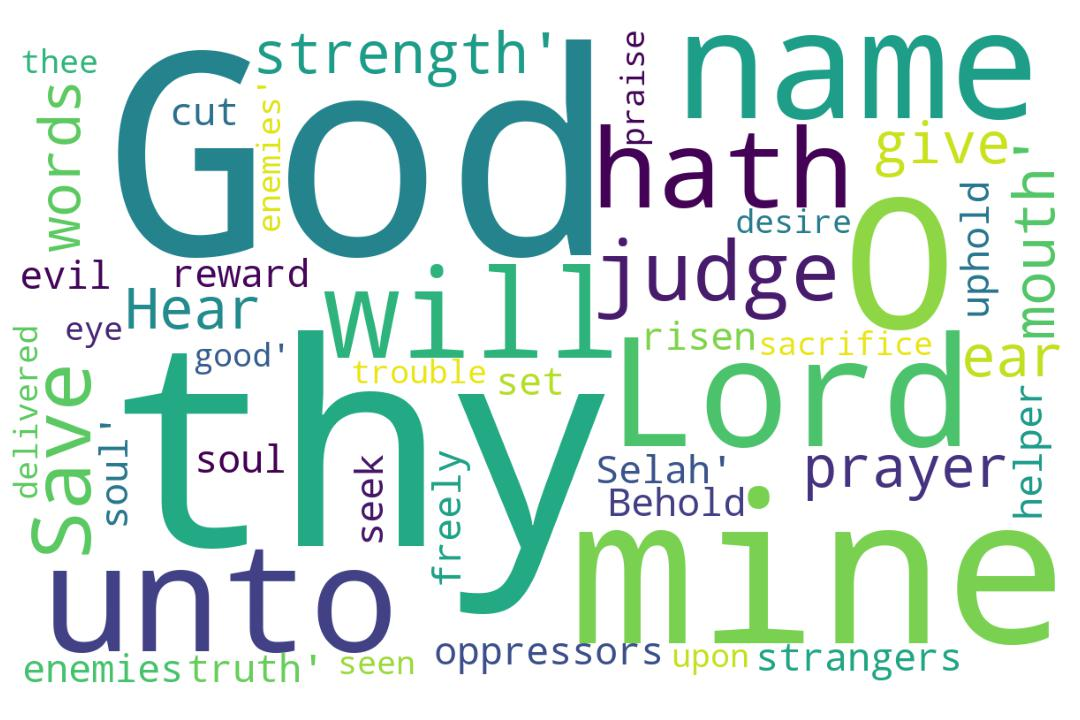
\includegraphics[width=\linewidth]{19OT-Psalms/Psalm54-WordCloud.jpg}
  \caption{Psalm 54 Word Cloud}
  \label{fig:Psalm 54 word Cloud}
\end{figure}

\marginpar{\scriptsize \centering \fcolorbox{bone}{lime}{\textbf{A PROMISED END}}\\ (Psalm 54:1-7) \begin{compactenum}[I.][8]
    \item God's \textbf{Fastidious Ear} \index[scripture]{Psalms!Psa 054:02}(Psa 54:2)
    \item A \textbf{Fearful Existence} \index[scripture]{Psalms!Psa 054:03}(Psa 54:3)
    \item \textbf{Fitting Evil} \index[scripture]{Psalms!Psa 054:05}(Psa 54:5)
    \item \textbf{Finished Enemies} \index[scripture]{Psalms!Psa 054:05}\index[scripture]{Psalms!Psa 054:06}(Psa 54:5, 6)
    \item \textbf{Focused Eyes} \index[scripture]{Psalms!Psa 054:05}\index[scripture]{Psalms!Psa 054:07}(Psa 54:7)
    \item The \textbf{Final End} \index[scripture]{Psalms!Psa 054:05}\index[scripture]{Psalms!Psa 054:07}(Psa 54:7)
\end{compactenum}}

\marginpar{\scriptsize \centering \fcolorbox{bone}{yellow}{\textbf{KNOWING THE DELIVERER}}\\ (Psalm 54:1-7) \begin{compactenum}[I.][8]
    \item There is \textbf{Earnest}  \index[scripture]{Psalms!Psa 054:02}(Psa 054:2)
    \item There is \textbf{Enmity}  \index[scripture]{Psalms!Psa 054:02}(Psa 054:2)
    \item There is an \textbf{Emergency}  \index[scripture]{Psalms!Psa 054:03}(Psa 054:3)
    \item There is \textbf{Evil}  in store for some \index[scripture]{Psalms!Psa 054:05}(Psa 054:5)
    \item There is \textbf{Excitement}  \index[scripture]{Psalms!Psa 054:06}(Psa 054:6)
    \item There is \textbf{Expectation}  \index[scripture]{Psalms!Psa 054:06}(Psa 054:6)
    \item There is an \textbf{Eye}  to behold the Deliverance \index[scripture]{Psalms!Psa 054:07}(Psa 054:7)
\end{compactenum}}


\footnote{\textcolor[rgb]{0.00,0.25,0.00}{\hyperlink{TOC}{Return to end of Table of Contents.}}}\footnote{\href{https://audiobible.com/bible/psalms_54.html}{\textcolor[cmyk]{0.99998,1,0,0}{Psalms Audio}}}\textcolor[cmyk]{0.99998,1,0,0}{To the chief Musician on Neginoth, Maschil, \emph{A Psalm} of David, when the Ziphims came and said to Saul, Doth not David hide himself with us?}\\
\\
\textcolor[cmyk]{0.99998,1,0,0}{Save me, O God, by thy name, and judge me by thy strength.}
[2] \textcolor[cmyk]{0.99998,1,0,0}{\fcolorbox{bone}{lime}{Hear} my prayer, O God; give ear to the words of my mouth.}
[3] \textcolor[cmyk]{0.99998,1,0,0}{For strangers are risen up against me, and oppressors seek after my soul: they have \fcolorbox{bone}{lime}{not set God before them}. Selah.}
[4] \textcolor[cmyk]{0.99998,1,0,0}{Behold, God \emph{is} mine helper: the Lord \emph{is} with them that uphold my soul.}
[5] \textcolor[cmyk]{0.99998,1,0,0}{He shall \fcolorbox{bone}{lime}{reward evil} unto mine \fcolorbox{bone}{lime}{enemies}: cut them off in thy truth.}
[6] \textcolor[cmyk]{0.99998,1,0,0}{I will freely sacrifice unto thee: I will praise thy name, O LORD; for \emph{it} \emph{is} good.}
[7] \textcolor[cmyk]{0.99998,1,0,0}{For he hath delivered me out of all trouble: and mine \fcolorbox{bone}{lime}{eye} hath seen \emph{his} \fcolorbox{bone}{lime}{\emph{desire}} upon mine enemies.}

